\chapter{トレースログ可視化ツール TraceLogVisualizer の実装}

\section{TraceLogVisualizerの全体像}

TLVの主機能は,2つの主たるプロセスと6種の外部ファイルによって実現される.
図\ref{fig:tlv}にTLVの全体像を示す.

2つの主たるプロセスとは,標準形式への変換と,図形データの生成である.
標準形式への変換は,任意の形式をもつトレースログを標準形式トレースログに変換する処理である.
この処理には外部ファイルとして変換元のトレースログファイル,リソースを定義したリソースファイル,リソースタイプを定義したリソースヘッダファイル,標準形式トレースログへの変換ルールを定義した変換ルールファイルが読み込まれる.

また,図形データの生成は,変換した標準形式トレースログに対して可視化ルールを適用し図形データを生成する処理である.
この処理には外部ファイルとして可視化ルールファイルが読み込まれる.
可視化ルールファイルとは図形と可視化ルールを定義したファイルである.

\begin{figure}[p]
\begin{center}
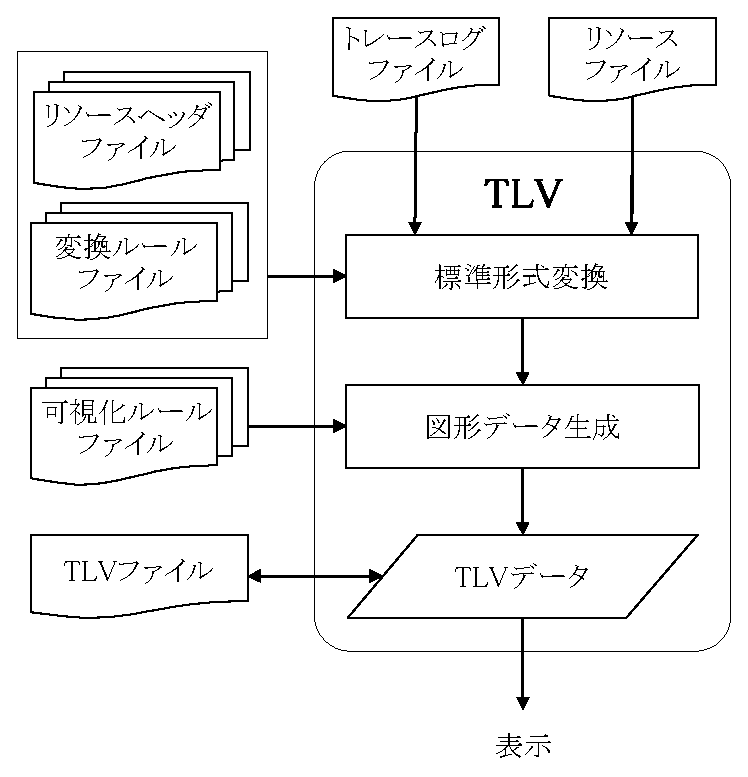
\includegraphics[scale=0.75]{img/tlv.eps}
\caption{TLVの全体像}
\label{fig:tlv}
\end{center}
\end{figure}

\section{TraceLogVisualizerのプロセス}

本節では,TLVの主たる2つのプロセスについて説明する.

\subsection{標準形式への変換}

標準形式トレースログへの変換は,トレースログファイルを先頭から行単位で読み込み,変換ルールファイルで定義される置換ルールに従い標準形式トレースログに置換していくことで行われる.変換ルールファイルの詳細は\ref{subsec:cnvFile}小節で説明する.

1つの置換ルールに対して複数の標準形式トレースログを出力可能である.
また,所望の標準形式トレースログに変換する際,トレースログファイルの情報だけでは足りない場合がある.

たとえば,TOPPERS/ASPカーネルというRTOSのトレースログを標準形式トレースログに変換することを考えてみる.
TOPPERS/ASPカーネルのトレースログを以下に示す.

\begin{EBNF}
[1000]task 1 becomes RUNNABLE
[1005]dispatch to task 1.
[1100]task 1 becomes WAITING
\end{EBNF}

上記のトレースログの内容を簡単に説明すると,時刻1000にタスクIDが1のタスクの状態がRUNNABLEになり,時刻1005に同タスクがディスパッチされ,時刻1100に同タスクの状態がWAITINGになったことを示している.

この場合,標準形式トレースログは次のように出力されることが要求される.
なお,説明のため簡略化しており,実際の変換結果とは異なる.

\begin{EBNF}
[1000]Task(id==1).activate()
[1000]Task(id==1).state = RUNNABLE
[1005]Task(state==RUNNING).state=RUNNABLE
[1005]Task(id==1).state = RUNNING
[1100]Task(id==1).state = WAITING
\end{EBNF}

元のトレースログが3行なのに対し,要求される標準形式トレースログは5行となっている.
これは,標準形式トレースログの1行目と3行目が状況により追加される必要があるからである.
標準形式トレースログの1行目は,元のトレースログの1行目に対応しており,起動(\verb|activate()|)というタスクの振る舞いを可視化したいという要求があるため追加される必要がある.
また,標準形式トレースログの3行目は,元のトレースログの2行目に対応しており,すでに起動しているタスクがプリエンプトされて状態がRUNNABLEになるという情報が元のトレースログに存在しないため追加される必要がある.
しかしながら,これら標準形式トレースログの追加が必要になるのは一定の条件下のみである.
標準形式トレースログの1行目は,タスクIDが1のタスクの状態が,時刻1000未満のときにDORMANTである場合だけである.
これは,起動という状態遷移を行うのが状態がDORMANTからRUNNABLEに遷移するときだけであり,状態がDORMANTになっただけでは起動であるのかどうか判断出来ないためである.
また,標準形式トレースログの3行目が必要なときは,時刻1005のときに状態がRUNNINGのタスクが存在する場合だけである.

このように,リソース属性の遷移に伴うイベントや,元のトレースログに欠落している情報を補うイベントなど,元のトレースログの情報だけでは判断出来ないイベントを出力するには,特定時刻における特定リソースの有無やその数,特定リソースの属性の値などの条件で出力を制御出来る必要がある.
そのため,TLVの変換ルールでは,置換する条件の指定と,条件指定の際に用いる情報を置換マクロを用いて取得できる仕組みを提供した.
具体的な記述例は\ref{subsec:cnvFile}小節で述べる.

標準形式トレースログに含まれるリソースは,リソースファイルで定義されていなければならない.
リソースファイルには,各リソースについてその名前とリソースタイプ,必要であれば各属性の初期値を定義する.
リソースファイルの詳細については\ref{subsec:resFile}小節で述べる.

また,その際に使用されるリソースタイプはリソースヘッダファイルで定義されていなければならない.
リソースヘッダファイルには各リソースタイプについて,その名前と属性,振る舞いの定義を記述する.
リソースヘッダファイルの詳細については\ref{subsec:reshFile}小節で述べる.

標準形式変換に用いる変換ルールファイルやリソースヘッダファイル,可視化ルールファイルはリソースファイルに記述する.

\subsection{図形データの生成}

標準形式変換プロセスを経て得られた標準形式トレースログは,可視化ルールファイルの定義に従い図形データを生成する.
読み込まれた標準形式トレースログは一行ずつ



\section{TraceLogVisualizerのインターフェイス}

\subsection{Json形式}

\subsection{トレースログファイル}

\subsection{リソースファイル}
\label{subsec:resFile}

\subsection{リソースヘッダファイル}
\label{subsec:reshFile}

\subsection{変換ルールファイル}
\label{subsec:cnvFile}

置換対象のトレースログは正規表現を用いて記述される.
正規表現内において名前付きグループ化構成体を用いると入力文字列中の部分文字列をキャプチャすることができ,置換の際に使用できるようになる.

\subsection{可視化ルールファイル}

\subsection{TLVファイル}

\section{TraceLogVisualizerの機能}